\tikzset{every picture/.style={line width=0.75pt}} %set default line width to 0.75pt        

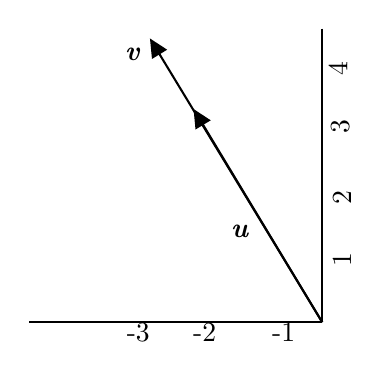
\begin{tikzpicture}[x=0.75pt,y=0.75pt,yscale=-1,xscale=1]
%uncomment if require: \path (0,218); %set diagram left start at 0, and has height of 218

%Shape: Boxed Line [id:dp4197928522176406] 
\draw    (296,5.29) -- (296,146.71) ;
%Shape: Boxed Line [id:dp2691398772595486] 
\draw    (296,146.71) -- (154.58,146.71) ;
%Straight Lines [id:da7555271225783102] 
\draw    (235.55,46.57) -- (296,146.71) ;
\draw [shift={(234,44)}, rotate = 58.88] [fill={rgb, 255:red, 0; green, 0; blue, 0 }  ][line width=0.08]  [draw opacity=0] (8.93,-4.29) -- (0,0) -- (8.93,4.29) -- cycle    ;
%Straight Lines [id:da3247719140034826] 
\draw    (296,146.71) -- (214.56,12.56) ;
\draw [shift={(213,10)}, rotate = 418.74] [fill={rgb, 255:red, 0; green, 0; blue, 0 }  ][line width=0.08]  [draw opacity=0] (8.93,-4.29) -- (0,0) -- (8.93,4.29) -- cycle    ;

% Text Node
\draw (298.87,52.5) node [anchor=north] [inner sep=0.75pt]  [rotate=-270] [align=left] {3};
% Text Node
\draw (299.88,86.5) node [anchor=north] [inner sep=0.75pt]  [rotate=-270] [align=left] {2};
% Text Node
\draw (299.88,116.5) node [anchor=north] [inner sep=0.75pt]  [rotate=-270] [align=left] {1};
% Text Node
\draw (277.38,146) node [anchor=north] [inner sep=0.75pt]   [align=left] {\mbox{-}1};
% Text Node
\draw (239.38,146) node [anchor=north] [inner sep=0.75pt]   [align=left] {\mbox{-}2};
% Text Node
\draw (207.38,146) node [anchor=north] [inner sep=0.75pt]   [align=left] {\mbox{-}3};
% Text Node
\draw (263,98.36) node [anchor=north east] [inner sep=0.75pt]   [align=left] {\textbf{\textit{u}}};
% Text Node
\draw (298,24.29) node [anchor=north] [inner sep=0.75pt]  [rotate=-270] [align=left] {4};
% Text Node
\draw (211,13) node [anchor=north east] [inner sep=0.75pt]   [align=left] {\textbf{\textit{v}}};


\end{tikzpicture}
